%----------------------------------------------------------------------------------------
%	PACKAGES AND DOCUMENT CONFIGURATIONS
%----------------------------------------------------------------------------------------
\documentclass[12pt,a4paper]{report}

\usepackage{geometry} % To set page size and margins accurately
\usepackage{siunitx} % Provides the \SI{}{} and \si{} command for typesetting SI units
\usepackage{graphicx} % Required for the inclusion of images
\usepackage{amsmath} % Required for some math elements 
\usepackage{paralist} % For compactitem lists
\usepackage{color} % Color management options
\usepackage{listings} % To typeset source code
\usepackage{pdflscape} % Landscape pages
\usepackage{acro} %To create acronyms lists
\usepackage{pgfplots}
\usepackage{tabu}
\usepackage{longtable}
\usepackage[strings]{underscore}
\usepackage{pdfpages}
\usepackage{hyperref}
\usepackage[backend=biber, style=ieee]{biblatex}
\usepackage{tikz}

\addbibresource{references.bib}

\geometry{
	a4paper,
	total={160mm,247mm},
	left=30mm,
	top=25mm
}
\setlength\parindent{0.5cm} % Set indentation for paragraphs
% To make floats, on float only pages, placed at top.
\makeatletter
	\setlength{\@fptop}{0pt}
	\setlength{\@fpbot}{0pt plus 1fil}
\makeatother

%----------------------------------------------------------------------------------------
%	ACRONYMS AND SYMBOLS
%----------------------------------------------------------------------------------------
% class `abbrev': abbreviations:
\DeclareAcronym{uc}{
	short = $\mu$C ,
	long  = Micro-Controller ,
	short-plural = s ,
	long-plural = s ,
	class = abbrev
}
\DeclareAcronym{sipo}{
	short = SIPO ,
	long  = Serial In Parallel Out ,
	class = abbrev
}
\DeclareAcronym{pcb}{
	short = PCB ,
	long  = Printed Circuit Board ,
	short-plural = 's ,
	long-plural = s ,
	class = abbrev
}
\DeclareAcronym{midi}{
	short = MIDI ,
	long  = Musical Instrument Digital Interface,
	class = abbrev
}
\DeclareAcronym{daw}{
	short = DAW ,
	long  = Digital Audio Workstation,
	short-plural = 's ,
	long-plural = s ,
	class = abbrev
}
\DeclareAcronym{usb}{
	short = USB ,
	long  = Universal Serial Bus,
	class = abbrev
}
\DeclareAcronym{spi}{
	short = SPI ,
	long  = Serial Peripheral Interface,
	class = abbrev
}
\DeclareAcronym{i2c}{
	short = I$^2$C ,
	long  = Inter-Integrated Circuit,
	class = abbrev
}
\DeclareAcronym{i2s}{
	short = I$^2$S ,
	long  = Inter-IC Sound,
	class = abbrev
}
\DeclareAcronym{ic}{
	short = IC ,
	long  = Integrated Circuit,
	short-plural = s ,
	long-plural = s ,
	class = abbrev
}
\DeclareAcronym{otg}{
	short = OTG ,
	long  = On The Go,
	class = abbrev
}
\DeclareAcronym{dac}{
	short = DAC ,
	long  = Digital to Analog Converter,
	short-plural = s ,
	long-plural = s ,
	class = abbrev
}
\DeclareAcronym{adc}{
	short = ADC ,
	long  = Analog to Digital Converter,
	short-plural = s ,
	long-plural = s ,
	class = abbrev
}
\DeclareAcronym{lcd}{
	short = LCD ,
	long  = Liquid Crystal Display,
	short-plural = s ,
	long-plural = s ,
	class = abbrev
}


%----------------------------------------------------------------------------------------
%	DOCUMENT INFORMATION AND TITLE PAGE
%----------------------------------------------------------------------------------------
\renewcommand{\thepage}{Cover}
\title{Simple Beat Matrix Drum Machine \\ using an ARM M4 CPU} % Title

\author{Pieter \textsc{Goos}} % Author name

\date{\today} % Date for the report

\makeatletter
\let\thetitle\@title
\let\theauthor\@author
\let\thedate\@date
\makeatother

\begin{document}

\begin{titlepage}
    \centering
    \vspace*{0.5 cm}
    
\includegraphics[scale = 2]{EELogo.png}\\[1.0 cm]   % University Logo
    \vspace{3cm}
    \rule{\linewidth}{0.2 mm} \\[0.4 cm]
    { \huge \bfseries \thetitle }\\[0.4 cm]
    \rule{\linewidth}{0.2 mm} \\[1.5 cm]
    \vspace{2cm}
	\begin{minipage}{6.5cm}
		\begin{flushleft} \large
			\emph{Student Name:}\\
			\emph{Student Number:}\\
			\emph{Study Leader:}\\
			\emph{Date:}
		\end{flushleft}
	\end{minipage}~
	\begin{minipage}{6.5cm}
		\begin{flushright} \large
		\theauthor\\
		19231466-2015\\
		Dr. Lourens Visagie\\
		May 2019
		\end{flushright}
	\end{minipage}\\[2 cm]
    \vfill
    
\includegraphics[width=7cm]{SUNLogo.jpg}\\[1.0 cm]
    Report submitted in partial fulfilment of the requirements of the module Project (E) 448 for the degree Baccalaureus in Engineering in the Department of Electrical and Electronic Engineering at the University of Stellenbosch.
    
\end{titlepage}

%----------------------------------------------------------------------------------------
%	Acknowledgements
%----------------------------------------------------------------------------------------
\pagenumbering{Roman}
\addcontentsline{toc}{chapter}{Preamble}
\addcontentsline{toc}{section}{Acknowledgements}
\section*{Acknowledgements}

\newpage

%----------------------------------------------------------------------------------------
%	DECLARATION
%----------------------------------------------------------------------------------------
\addcontentsline{toc}{section}{Plagiarism Declaration}
\section*{Plagiarism Declaration / Plagiaatverklaring}
\begin{enumerate}
\item Plagiarism is the use of ideas, material and other intellectual property of another's work and to present is as my own. \newline \textit{Plagiaat is die oorneem en gebruik van die idees, materiaal en ander intellektuele eiendom van ander persone asof dit jou eie werk is.} 
\item I agree that plagiarism is a punishable offence because it constitutes theft. \newline \textit{Ek erken dat die pleeg van plagiaat 'n strafbare oortreding is aangesien dit ‘n vorm van diefstal is. }
\item I also understand that direct translations are plagiarism. \newline \textit{Ek verstaan ook dat direkte vertalings plagiaat is. }
\item Accordingly all quotations and contributions from any source whatsoever (including the internet) have been cited fully. I understand that the reproduction of text without quotation marks (even when the source is cited) is plagiarism. \newline \textit{Dienooreenkomstig is alle aanhalings en bydraes vanuit enige bron (ingesluit die internet) volledig verwys (erken). Ek erken dat die woordelikse aanhaal van teks sonder aanhalingstekens (selfs al word die bron volledig erken) plagiaat is. }
\item I declare that the work contained in this assignment, except where otherwise stated, is my original work and that I have not previously (in its entirety or in part) submitted it for grading in this module/assignment or another module/assignment. \newline \textit{Ek verklaar dat die werk in hierdie skryfstuk vervat, behalwe waar anders aangedui, my eie oorspronklike werk is en dat ek dit nie vantevore in die geheel of gedeeltelik ingehandig het vir bepunting in hierdie module/werkstuk of ‘n ander module/werkstuk nie.} 
\end{enumerate}
\vspace{1cm}
\begin{table}[ht]
	\begin{center}
		\begin{tabular*}{15.5cm}{@{\extracolsep{\fill}}lll}
			\makebox[8cm]{\hrulefill} & & \makebox[6cm]{\hrulefill}\\
			%\hrulefill & & \hrulefill \\
			Signature & & Student number \\
			\textit{Handtekening} & & \textit{Studentenommer} \\[1cm]
		    \makebox[8cm]{\hrulefill} & & \makebox[6cm]{\hrulefill}\\ 
			%\hrulefill & & \hrulefill\\
			Initials and surname & & Date \\
			\textit{Voorletters en van} & & \textit{Datum}\\
		\end{tabular*}
	\end{center}
\end{table}
\newpage

%----------------------------------------------------------------------------------------
%	Summary
%----------------------------------------------------------------------------------------
\addcontentsline{toc}{section}{Summary / Opsomming}
\section*{Summary}
\section*{Opsomming}


\newpage

%----------------------------------------------------------------------------------------
%	TOC, Lists (Figures, Tables etc)
%----------------------------------------------------------------------------------------
\tableofcontents
\listoffigures
\listoftables
%Acronym lists
\printacronyms[name={List of Abbreviations}]
\newpage

%----------------------------------------------------------------------------------------
%	SECTION 1
%----------------------------------------------------------------------------------------
\pagenumbering{arabic}
\chapter{Introduction}
\section{Project Background}
\section{Project Aims}

%----------------------------------------------------------------------------------------
%	SECTION 2
%----------------------------------------------------------------------------------------
\chapter{Literature Study}
To design a drum machine one must first determine what that is and could be. Unfortunately it is not as clean cut as one would believe as there are many types of drum machines. The complexity and mere perception of what it is has changed since its beginnings in the 1930s, thus a point in time will need be chosen to be the basis of this project.
\section{The Beginning of Drum Machines}
Before drum machines could be programmed to the musician's liking it would make simple or pre-recorded sounds on a schedule. This meant that the \textit{drum machines} of the time, the 1930s into the 1950s, acted mostly as timing to be used in conjunction with other instruments \cite{rhythmart}. \\
The earliest device one could conceive as a drum machine was the \textit{Rhythmicon} by L\'eon Theremin and commissioned by Henry Cowell \cite{rhythmart, beatgoeson}. The \textit{Rhythmicon} was completed in 1931 and could only produce 16 different rhythms \cite{schedel}. These rhythms would all be more rapid than the previous, all based on a periodic base rhythm. This device would, however, only act as a concept for the next two decades. \\
In the late 1950s large devices such as the \textit{Chamberlin Rhythmate} or the \textit{Wurlitzer Sideman} came on the market. These two offered a more pleasant sound to listen to by playing back audio tapes (at various speeds), and a system similar to a music box respectively \cite{rhythmart, beatgoeson}. The latter, the \textit{Sideman}, had rhythms styles including the Samba, Waltz and more\cite{WangOliver2014Htdm}. \\
Moving into the 1960s drum machines started to be manufactured with the, at the time, new solid-state transistors. These transistors allowed for the units to shrink in size drastically. In Japan a new trend was pushed by companies such as Ace Tone, and Keio-Giken to create organ accessories. Outside of Japan the idea would be taken in a different direction by creating pre-set rhythm boxes, such as the \textit{Elka Drummer One}. For these devices to progress, a new level of control would be needed \cite{rhythmart}.
\section{Programmable Drum Machines}
First one has to understand what is meant by \textit{programmable}: this refers to the ability for musicians to create their own patterns of internal sounds.\\
\begin{figure}[h!]
	\begin{center}
		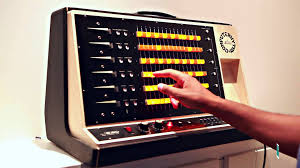
\includegraphics[width = 0.5\textwidth, angle=0, origin=c]{computerhythm.jpg}
		\caption{An Eko Compute Rhythm in Use \cite{comprhythImg}}
		\label{fig:comprhyt}
	\end{center}
\end{figure}
The first programmable drum machines came about in the 1970s with the \textit{Eko Compute Rhythm} in 1972, as seen in Figure \ref{fig:comprhyt}. This product featured a beat matrix, something that can still be found today \cite{beatgoeson}. Beat Matrices will be discussed in Section \ref{sec:beatmatrix}. Roland came out with the first drum machine to feature a microprocessor in 1978 with the \textit{CR-78 CompuRhythm}. This allowed the user to store entire sequences \cite{cr78}. Several years down the line they brought out the \textit{TR-808} with a set of programmable synthesized analogue sounds \cite{tr808, beatgoeson}. At this point the desire for real drum sounds was high and thus came the Sample-Based Drum Machines.\\
In 1980 the \textit{Linn Electronics LM-1} was released to be the first drum machine to use recorded samples as opposed to synthesized sounds \cite{beatgoeson}. Synth manufacturers began to enter the rhythmic device market with product that made use of swappable memory cards, had \ac{midi} integration, among other features \cite{rhythmart}.\\
The most important feature to be added in the coming years was being able to sample sounds on the device itself. This was pioneered by the \textit{Akai MPC} series of drum machines. These featured 16 responsive pad controllers and had all the features of a drum machine \cite{beatgoeson, rhythmart}. This wave of new machines throughout the 1980s paved the way for stations such as the more recent \textit{Native Instruments Maschine} series \cite{rhythmart}, an example of which can be seen in Figure \ref{fig:maschine}.\\
\begin{figure}[h!]
	\begin{center}
		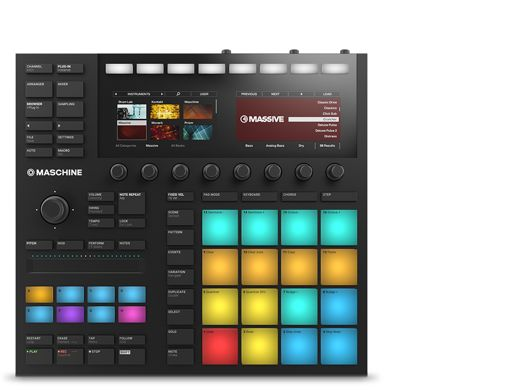
\includegraphics[width = 0.3\textwidth, angle=0, origin=c, trim={0 0 140px 35px}, clip]{maschine.jpg}
		\caption{Native Instruments Maschine Mk3 \cite{maschine}}
		\label{fig:maschine}
	\end{center}
\end{figure}


%----------------------------------------------------------------------------------------
%	SECTION 3
%----------------------------------------------------------------------------------------
\chapter{Hardware Design}

\begin{figure}
\tikzset{every picture/.style={line width=0.75pt}} %set default line width to 0.75pt        

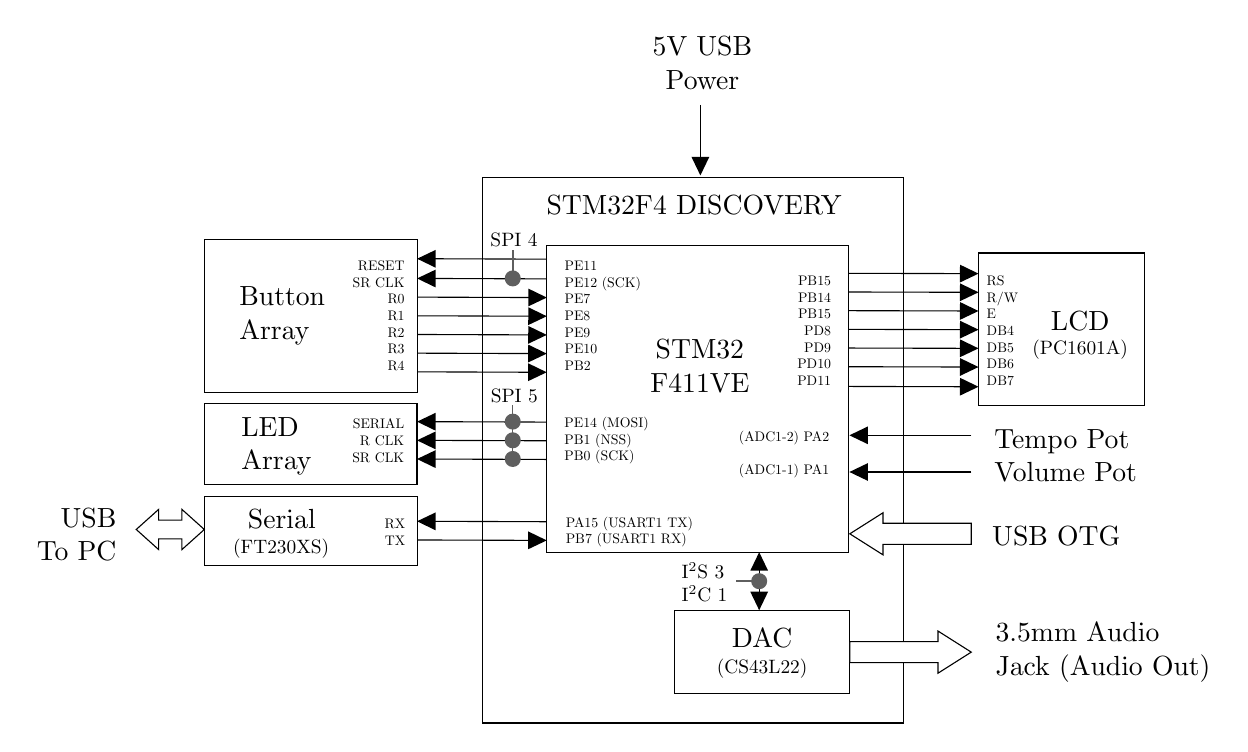
\begin{tikzpicture}[x=0.75pt,y=0.75pt,yscale=-1,xscale=1]
%uncomment if require: \path (0,481); %set diagram left start at 0, and has height of 481

%Shape: Rectangle [id:dp5918076160842385] 
\draw   (230,97) -- (433,97) -- (433,360) -- (230,360) -- cycle ;
%Shape: Rectangle [id:dp0432000596696005] 
\draw   (322.5,306) -- (406.98,306) -- (406.98,346) -- (322.5,346) -- cycle ;
%Shape: Rectangle [id:dp7985098815357947] 
\draw   (261,130) -- (406.5,130) -- (406.5,278) -- (261,278) -- cycle ;
%Right Arrow [id:dp2315359222828235] 
\draw  [fill={rgb, 255:red, 255; green, 255; blue, 255 }  ,fill opacity=1 ] (407,320.79) -- (449.5,320.79) -- (449.5,315.71) -- (465.5,325.86) -- (449.5,336) -- (449.5,330.93) -- (407,330.93) -- cycle ;
%Straight Lines [id:da20381712216745096] 
\draw    (363.33,279.7) -- (363.33,303.67) ;
\draw [shift={(363.33,305.67)}, rotate = 270] [fill={rgb, 255:red, 0; green, 0; blue, 0 }  ][line width=0.75]  [draw opacity=0] (8.93,-4.29) -- (0,0) -- (8.93,4.29) -- cycle    ;
\draw [shift={(363.33,277.7)}, rotate = 90] [fill={rgb, 255:red, 0; green, 0; blue, 0 }  ][line width=0.75]  [draw opacity=0] (8.93,-4.29) -- (0,0) -- (8.93,4.29) -- cycle    ;
%Right Arrow [id:dp9428678654929861] 
\draw  [fill={rgb, 255:red, 255; green, 255; blue, 255 }  ,fill opacity=1 ] (465.5,273.93) -- (423,273.93) -- (423,279) -- (407,268.86) -- (423,258.71) -- (423,263.79) -- (465.5,263.79) -- cycle ;
%Straight Lines [id:da6753000057653133] 
\draw    (465.5,239.07) -- (408.8,239.07) ;
\draw [shift={(406.8,239.07)}, rotate = 360] [fill={rgb, 255:red, 0; green, 0; blue, 0 }  ][line width=0.75]  [draw opacity=0] (8.93,-4.29) -- (0,0) -- (8.93,4.29) -- cycle    ;

%Straight Lines [id:da7619363353708244] 
\draw [color={rgb, 255:red, 0; green, 0; blue, 0 }  ,draw opacity=1 ]   (465.5,221.4) -- (408.8,221.4) ;
\draw [shift={(406.8,221.4)}, rotate = 360] [fill={rgb, 255:red, 0; green, 0; blue, 0 }  ,fill opacity=1 ][line width=0.75]  [draw opacity=0] (8.93,-4.29) -- (0,0) -- (8.93,4.29) -- cycle    ;

%Straight Lines [id:da15096112605281875] 
\draw    (406.5,188.35) -- (467,188.5) ;
\draw [shift={(469,188.5)}, rotate = 180.14] [fill={rgb, 255:red, 0; green, 0; blue, 0 }  ][line width=0.75]  [draw opacity=0] (8.93,-4.29) -- (0,0) -- (8.93,4.29) -- cycle    ;

%Straight Lines [id:da6435790607323693] 
\draw    (406.5,179.35) -- (467,179.5) ;
\draw [shift={(469,179.5)}, rotate = 180.14] [fill={rgb, 255:red, 0; green, 0; blue, 0 }  ][line width=0.75]  [draw opacity=0] (8.93,-4.29) -- (0,0) -- (8.93,4.29) -- cycle    ;

%Straight Lines [id:da7889393535599036] 
\draw    (406.5,170.35) -- (467,170.5) ;
\draw [shift={(469,170.5)}, rotate = 180.14] [fill={rgb, 255:red, 0; green, 0; blue, 0 }  ][line width=0.75]  [draw opacity=0] (8.93,-4.29) -- (0,0) -- (8.93,4.29) -- cycle    ;

%Straight Lines [id:da6837607975654587] 
\draw    (406.5,161.35) -- (467,161.5) ;
\draw [shift={(469,161.5)}, rotate = 180.14] [fill={rgb, 255:red, 0; green, 0; blue, 0 }  ][line width=0.75]  [draw opacity=0] (8.93,-4.29) -- (0,0) -- (8.93,4.29) -- cycle    ;

%Straight Lines [id:da865188420352889] 
\draw    (406.5,152.35) -- (467,152.5) ;
\draw [shift={(469,152.5)}, rotate = 180.14] [fill={rgb, 255:red, 0; green, 0; blue, 0 }  ][line width=0.75]  [draw opacity=0] (8.93,-4.29) -- (0,0) -- (8.93,4.29) -- cycle    ;

%Straight Lines [id:da2449046730837665] 
\draw    (406.5,143.35) -- (467,143.5) ;
\draw [shift={(469,143.5)}, rotate = 180.14] [fill={rgb, 255:red, 0; green, 0; blue, 0 }  ][line width=0.75]  [draw opacity=0] (8.93,-4.29) -- (0,0) -- (8.93,4.29) -- cycle    ;

%Straight Lines [id:da2794456064676478] 
\draw    (406.5,197.85) -- (467,198) ;
\draw [shift={(469,198)}, rotate = 180.14] [fill={rgb, 255:red, 0; green, 0; blue, 0 }  ][line width=0.75]  [draw opacity=0] (8.93,-4.29) -- (0,0) -- (8.93,4.29) -- cycle    ;

%Shape: Rectangle [id:dp2417461204409681] 
\draw   (469,133.57) -- (549,133.57) -- (549,207.23) -- (469,207.23) -- cycle ;
%Straight Lines [id:da008963581922469599] 
\draw    (261.02,146.03) -- (200.52,145.82) ;
\draw [shift={(198.52,145.82)}, rotate = 360.2] [fill={rgb, 255:red, 0; green, 0; blue, 0 }  ][line width=0.75]  [draw opacity=0] (8.93,-4.29) -- (0,0) -- (8.93,4.29) -- cycle    ;

%Straight Lines [id:da7017501912001678] 
\draw    (259.01,155.03) -- (198.51,154.82) ;

\draw [shift={(261.01,155.03)}, rotate = 180.2] [fill={rgb, 255:red, 0; green, 0; blue, 0 }  ][line width=0.75]  [draw opacity=0] (8.93,-4.29) -- (0,0) -- (8.93,4.29) -- cycle    ;
%Straight Lines [id:da6133179873808812] 
\draw    (259,164.03) -- (198.5,163.82) ;

\draw [shift={(261,164.03)}, rotate = 180.2] [fill={rgb, 255:red, 0; green, 0; blue, 0 }  ][line width=0.75]  [draw opacity=0] (8.93,-4.29) -- (0,0) -- (8.93,4.29) -- cycle    ;
%Straight Lines [id:da38787523560372406] 
\draw    (258.99,173.03) -- (198.49,172.82) ;

\draw [shift={(260.99,173.03)}, rotate = 180.2] [fill={rgb, 255:red, 0; green, 0; blue, 0 }  ][line width=0.75]  [draw opacity=0] (8.93,-4.29) -- (0,0) -- (8.93,4.29) -- cycle    ;
%Straight Lines [id:da049319380388482825] 
\draw    (258.98,182.03) -- (198.48,181.82) ;

\draw [shift={(260.98,182.03)}, rotate = 180.2] [fill={rgb, 255:red, 0; green, 0; blue, 0 }  ][line width=0.75]  [draw opacity=0] (8.93,-4.29) -- (0,0) -- (8.93,4.29) -- cycle    ;
%Straight Lines [id:da747407414364454] 
\draw    (258.97,191.03) -- (198.47,190.82) ;

\draw [shift={(260.97,191.03)}, rotate = 180.2] [fill={rgb, 255:red, 0; green, 0; blue, 0 }  ][line width=0.75]  [draw opacity=0] (8.93,-4.29) -- (0,0) -- (8.93,4.29) -- cycle    ;
%Straight Lines [id:da5651387140870967] 
\draw    (261.03,136.53) -- (200.53,136.32) ;
\draw [shift={(198.53,136.32)}, rotate = 360.2] [fill={rgb, 255:red, 0; green, 0; blue, 0 }  ][line width=0.75]  [draw opacity=0] (8.93,-4.29) -- (0,0) -- (8.93,4.29) -- cycle    ;

%Shape: Rectangle [id:dp8694052933297145] 
\draw   (96.2,126.97) -- (198.5,126.97) -- (198.5,200.63) -- (96.2,200.63) -- cycle ;
%Straight Lines [id:da2504593501522252] 
\draw    (260.98,263.03) -- (200.48,262.82) ;
\draw [shift={(198.48,262.82)}, rotate = 360.2] [fill={rgb, 255:red, 0; green, 0; blue, 0 }  ][line width=0.75]  [draw opacity=0] (8.93,-4.29) -- (0,0) -- (8.93,4.29) -- cycle    ;

%Straight Lines [id:da13433373243842728] 
\draw    (258.97,272.03) -- (198.47,271.82) ;

\draw [shift={(260.97,272.03)}, rotate = 180.2] [fill={rgb, 255:red, 0; green, 0; blue, 0 }  ][line width=0.75]  [draw opacity=0] (8.93,-4.29) -- (0,0) -- (8.93,4.29) -- cycle    ;
%Shape: Rectangle [id:dp8665495313374194] 
\draw   (96.2,251) -- (198.5,251) -- (198.5,284.2) -- (96.2,284.2) -- cycle ;
%Straight Lines [id:da01047939684415633] 
\draw    (260.99,215.03) -- (200.49,214.82) ;
\draw [shift={(198.49,214.82)}, rotate = 360.2] [fill={rgb, 255:red, 0; green, 0; blue, 0 }  ][line width=0.75]  [draw opacity=0] (8.93,-4.29) -- (0,0) -- (8.93,4.29) -- cycle    ;

%Straight Lines [id:da30157272917946076] 
\draw    (260.98,224.03) -- (200.48,223.82) ;
\draw [shift={(198.48,223.82)}, rotate = 360.2] [fill={rgb, 255:red, 0; green, 0; blue, 0 }  ][line width=0.75]  [draw opacity=0] (8.93,-4.29) -- (0,0) -- (8.93,4.29) -- cycle    ;

%Straight Lines [id:da6459450622816814] 
\draw    (260.97,233.03) -- (200.47,232.82) ;
\draw [shift={(198.47,232.82)}, rotate = 360.2] [fill={rgb, 255:red, 0; green, 0; blue, 0 }  ][line width=0.75]  [draw opacity=0] (8.93,-4.29) -- (0,0) -- (8.93,4.29) -- cycle    ;

%Shape: Rectangle [id:dp9252289543251917] 
\draw   (96.2,205.88) -- (198.47,205.88) -- (198.47,244.98) -- (96.2,244.98) -- cycle ;
%Left Right Arrow [id:dp964472909485768] 
\draw   (63.2,266.77) -- (74,257.08) -- (74,262.28) -- (85.2,262.28) -- (85.2,257.08) -- (96,266.77) -- (85.2,276.46) -- (85.2,271.26) -- (74,271.26) -- (74,276.46) -- cycle ;
%Straight Lines [id:da39718515123626186] 
\draw    (335,62.2) -- (335,94.2) ;
\draw [shift={(335,96.2)}, rotate = 270] [fill={rgb, 255:red, 0; green, 0; blue, 0 }  ][line width=0.75]  [draw opacity=0] (8.93,-4.29) -- (0,0) -- (8.93,4.29) -- cycle    ;

%Straight Lines [id:da06860468568514189] 
\draw [color={rgb, 255:red, 95; green, 95; blue, 95 }  ,draw opacity=1 ][line width=0.75]    (244.6,132.18) -- (244.6,145.8) ;
\draw [shift={(244.6,145.8)}, rotate = 90] [color={rgb, 255:red, 95; green, 95; blue, 95 }  ,draw opacity=1 ][fill={rgb, 255:red, 95; green, 95; blue, 95 }  ,fill opacity=1 ][line width=0.75]      (0, 0) circle [x radius= 3.35, y radius= 3.35]   ;

%Straight Lines [id:da4751452819167077] 
\draw [color={rgb, 255:red, 95; green, 95; blue, 95 }  ,draw opacity=1 ]   (244.6,208.58) -- (244.6,232.8) ;
\draw [shift={(244.6,232.8)}, rotate = 90] [color={rgb, 255:red, 95; green, 95; blue, 95 }  ,draw opacity=1 ][fill={rgb, 255:red, 95; green, 95; blue, 95 }  ,fill opacity=1 ][line width=0.75]      (0, 0) circle [x radius= 3.35, y radius= 3.35]   ;

%Straight Lines [id:da6406994555027319] 
\draw [color={rgb, 255:red, 95; green, 95; blue, 95 }  ,draw opacity=1 ]   (244.6,216.03) -- (244.6,223.8) ;
\draw [shift={(244.6,223.8)}, rotate = 90] [color={rgb, 255:red, 95; green, 95; blue, 95 }  ,draw opacity=1 ][fill={rgb, 255:red, 95; green, 95; blue, 95 }  ,fill opacity=1 ][line width=0.75]      (0, 0) circle [x radius= 3.35, y radius= 3.35]   ;

%Straight Lines [id:da9004528527180191] 
\draw [color={rgb, 255:red, 95; green, 95; blue, 95 }  ,draw opacity=1 ]   (244.6,207.03) -- (244.6,214.8) ;
\draw [shift={(244.6,214.8)}, rotate = 90] [color={rgb, 255:red, 95; green, 95; blue, 95 }  ,draw opacity=1 ][fill={rgb, 255:red, 95; green, 95; blue, 95 }  ,fill opacity=1 ][line width=0.75]      (0, 0) circle [x radius= 3.35, y radius= 3.35]   ;

%Straight Lines [id:da4193219413571099] 
\draw [color={rgb, 255:red, 95; green, 95; blue, 95 }  ,draw opacity=1 ][line width=0.75]    (352.25,291.68) -- (363.33,291.68) ;
\draw [shift={(363.33,291.68)}, rotate = 0] [color={rgb, 255:red, 95; green, 95; blue, 95 }  ,draw opacity=1 ][fill={rgb, 255:red, 95; green, 95; blue, 95 }  ,fill opacity=1 ][line width=0.75]      (0, 0) circle [x radius= 3.35, y radius= 3.35]   ;


% Text Node
\draw (332,110.5) node  [align=left] {STM32F4 DISCOVERY};
% Text Node
\draw (336,42) node  [align=center] {5V USB \\Power};
% Text Node
\draw (364.74,319) node  [align=left] {DAC};
% Text Node
\draw (334.75,188) node  [align=center] {STM32\\F411VE};
% Text Node
\draw (529,326) node  [align=left] {3.5mm Audio\\Jack (Audio Out)};
% Text Node
\draw (506.5,270) node  [align=left] {USB OTG};
% Text Node
\draw (511,231) node  [align=left] {Tempo Pot\\Volume Pot};
% Text Node
\draw (518,166.4) node  [align=left] {LCD};
% Text Node
\draw (480.5,171) node [scale=0.5] [align=left] {RS\\R/W\\E\\DB4\\DB5\\DB6\\DB7};
% Text Node
\draw (389.83,171) node [scale=0.5] [align=right] {PB15\\PB14\\PB15\\PD8\\PD9\\PD10\\PD11};
% Text Node
\draw (375.33,230.5) node [scale=0.5] [align=right] {(ADC1-2) PA2\\\\(ADC1-1) PA1};
% Text Node
\draw (133.5,163.8) node  [align=left] {Button\\Array};
% Text Node
\draw (180,163.8) node [scale=0.5] [align=right] {RESET\\SR CLK\\R0\\R1\\R2\\R3\\R4};
% Text Node
\draw (288,163.8) node [scale=0.5] [align=left] {PE11\\PE12 (SCK)\\PE7\\PE8\\PE9\\PE10\\PB2};
% Text Node
\draw (133.35,261.6) node  [align=left] {Serial};
% Text Node
\draw (300.8,268) node [scale=0.5] [align=left] {PA15 (USART1 TX)\\PB7 (USART1 RX)};
% Text Node
\draw (187.8,268) node [scale=0.5] [align=right] {RX\\TX};
% Text Node
\draw (179.8,224) node [scale=0.5] [align=right] {SERIAL\\R CLK\\SR CLK};
% Text Node
\draw (130.75,226.5) node  [align=left] {LED\\Array};
% Text Node
\draw (289.8,224) node [scale=0.5] [align=left] {PE14 (MOSI)\\PB1 (NSS)\\PB0 (SCK)};
% Text Node
\draw (133,276) node [scale=0.7] [align=left] {(FT230XS)};
% Text Node
\draw (34.5,269.35) node  [align=right] {USB\\To PC};
% Text Node
\draw (518,180) node [scale=0.7] [align=left] {(PC1601A)};
% Text Node
\draw (337,292) node [scale=0.7] [align=left] {I$^2$S 3\\I$^2$C 1};
% Text Node
\draw (245.22,127.31) node [scale=0.7] [align=left] {SPI 4};
% Text Node
\draw (245.36,202.61) node [scale=0.7] [align=left] {SPI 5};
% Text Node
\draw (364.74,334) node [scale=0.7] [align=left] {(CS43L22)};


\end{tikzpicture}

\caption{Complete System Diagram}
\end{figure}

\section{\ac{uc}}
Before even being able to design the circuit as a whole the main controller needs to be chosen. To 
\section{LED Matrix Driver}

\subsection{Other}
To drive the LED matrix of 16 columns by 5 rows a circuit with shift registers is used. These shift registers will be \ac{sipo} so that the micro-controller can communicate in serial to the matrix. Three shift registers will be hooked up in series allowing for the serial signal to be passed from one \ac{ic} to the next. To conserve the amount of pins needed on the micro-controller both the rows and columns will be controlled by one serial signal. To further update the shift registers two clock signals are required. One for the Shift Register and another for the Register. \\
The chosen \acp{ic} are the 74HC595 latched shift registers and the ULN2803A Darlington transistor arrays. In conjunction, these 
\section{Button Matrix Driver}
\section{Tempo and Volume Control with LCD}

%----------------------------------------------------------------------------------------
%	SECTION 4
%----------------------------------------------------------------------------------------
\chapter{Software Design}

%----------------------------------------------------------------------------------------
%	SECTION 5
%----------------------------------------------------------------------------------------
\chapter{Conclusions and Recommendations}

%----------------------------------------------------------------------------------------
%	BIBLIOGRAPHY
%----------------------------------------------------------------------------------------
\printbibliography

%----------------------------------------------------------------------------------------

%----------------------------------------------------------------------------------------
%	APPENDIX
%----------------------------------------------------------------------------------------
\appendix
\chapter{Project Planning Schedule}

\chapter{ECSA Outcome Compliance}

\begin{longtable}[c]{|m{0.4\textwidth}|m{0.6\textwidth}|}
	\hline
	\multicolumn{1}{|c|}{\textbf{ECSA ELO}} & \multicolumn{1}{c|}{\textbf{Compliance}} \\
	\hline
	\endhead
	
	
	\textbf{ELO 1. Problem solving:} \newline Identify, formulate, analyse and solve complex engineering problems creatively and innovatively.&  \\
	\hline
	\textbf{ELO 2. Application of scientific and engineering knowledge:} \newline Apply knowledge of mathematics, natural sciences, engineering fundamentals and an engineering speciality to solve complex engineering problems.&  \\
	\hline
	\textbf{ELO 3. Engineering Design:} \newline Perform creative, procedural and non‐procedural design and synthesis of components, systems, engineering works, products or processes.&  \\
	\hline
	\textbf{ELO 4. Investigations, experiments and data analysis:} \newline Demonstrate competence to design and conduct investigations and experiments. &  \\
	\hline
	\textbf{ELO 5. Engineering methods, skills and tools, including Information Technology:} \newline Demonstrate competence to use appropriate engineering methods, skills and tools, including those based on information technology.&  \\
	\hline
	\textbf{ELO 6. Professional and technical communication:} \newline Demonstrate competence to communicate effectively, both orally and in writing, with engineering audiences and the community at large.&  \\
	\hline
	\textbf{ELO 8. Individual work:} \newline Demonstrate competence to work effectively as an individual.&  \\
	\hline
	\textbf{ELO 9. Independent Learning Ability:} \newline Demonstrate competence to engage in independent learning through well-developed learning skills.&  \\
	\hline
	
	\caption{ECSA ELO Compliance}
	\label{tab:ecsa}%
\end{longtable}%
	
\chapter{Circuit Diagram}
\begin{figure}[h!]
\begin{center}
	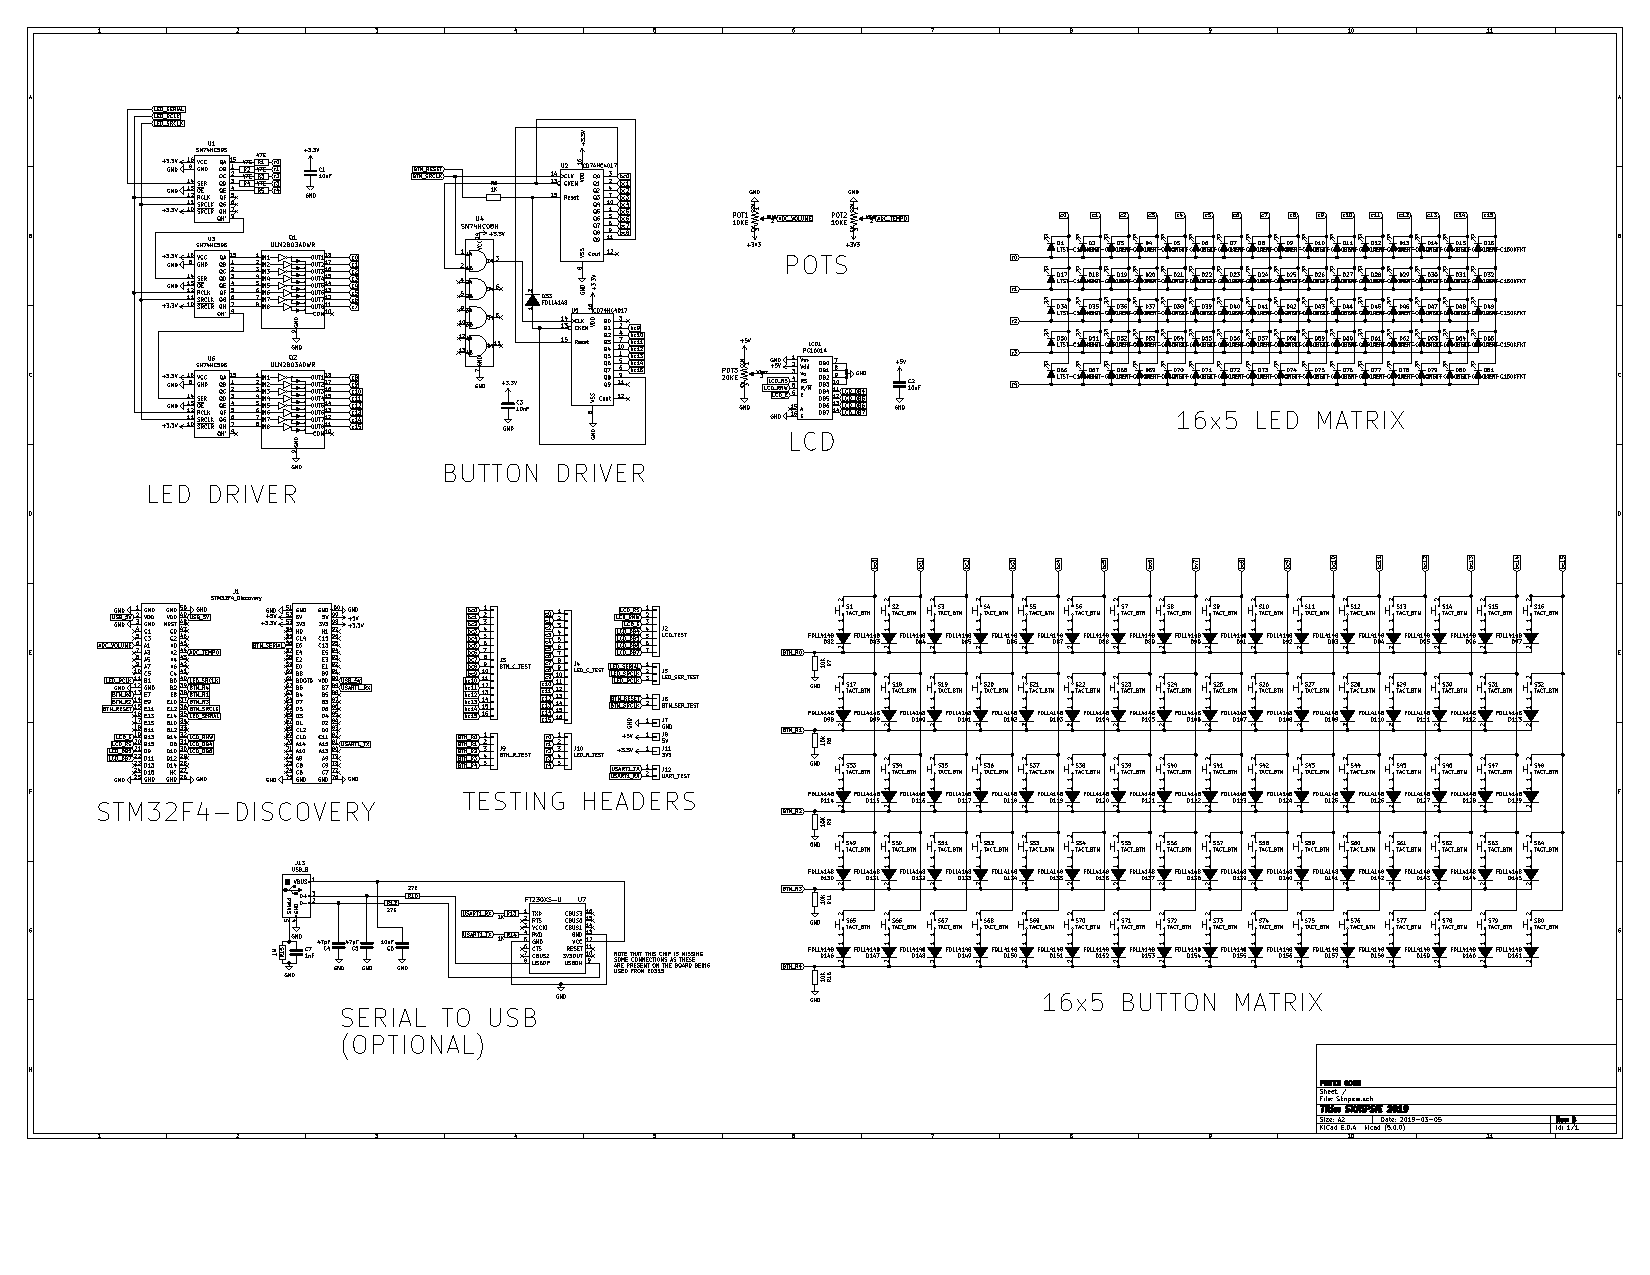
\includegraphics[width = \textwidth, angle=0, origin=c]{../Skripsie/Layout_05032019.pdf}
	\caption{The Final Revision (Rev. B) of the Circuit Diagram}
\end{center}
\end{figure}
\begin{figure}[h!]
	\begin{center}
		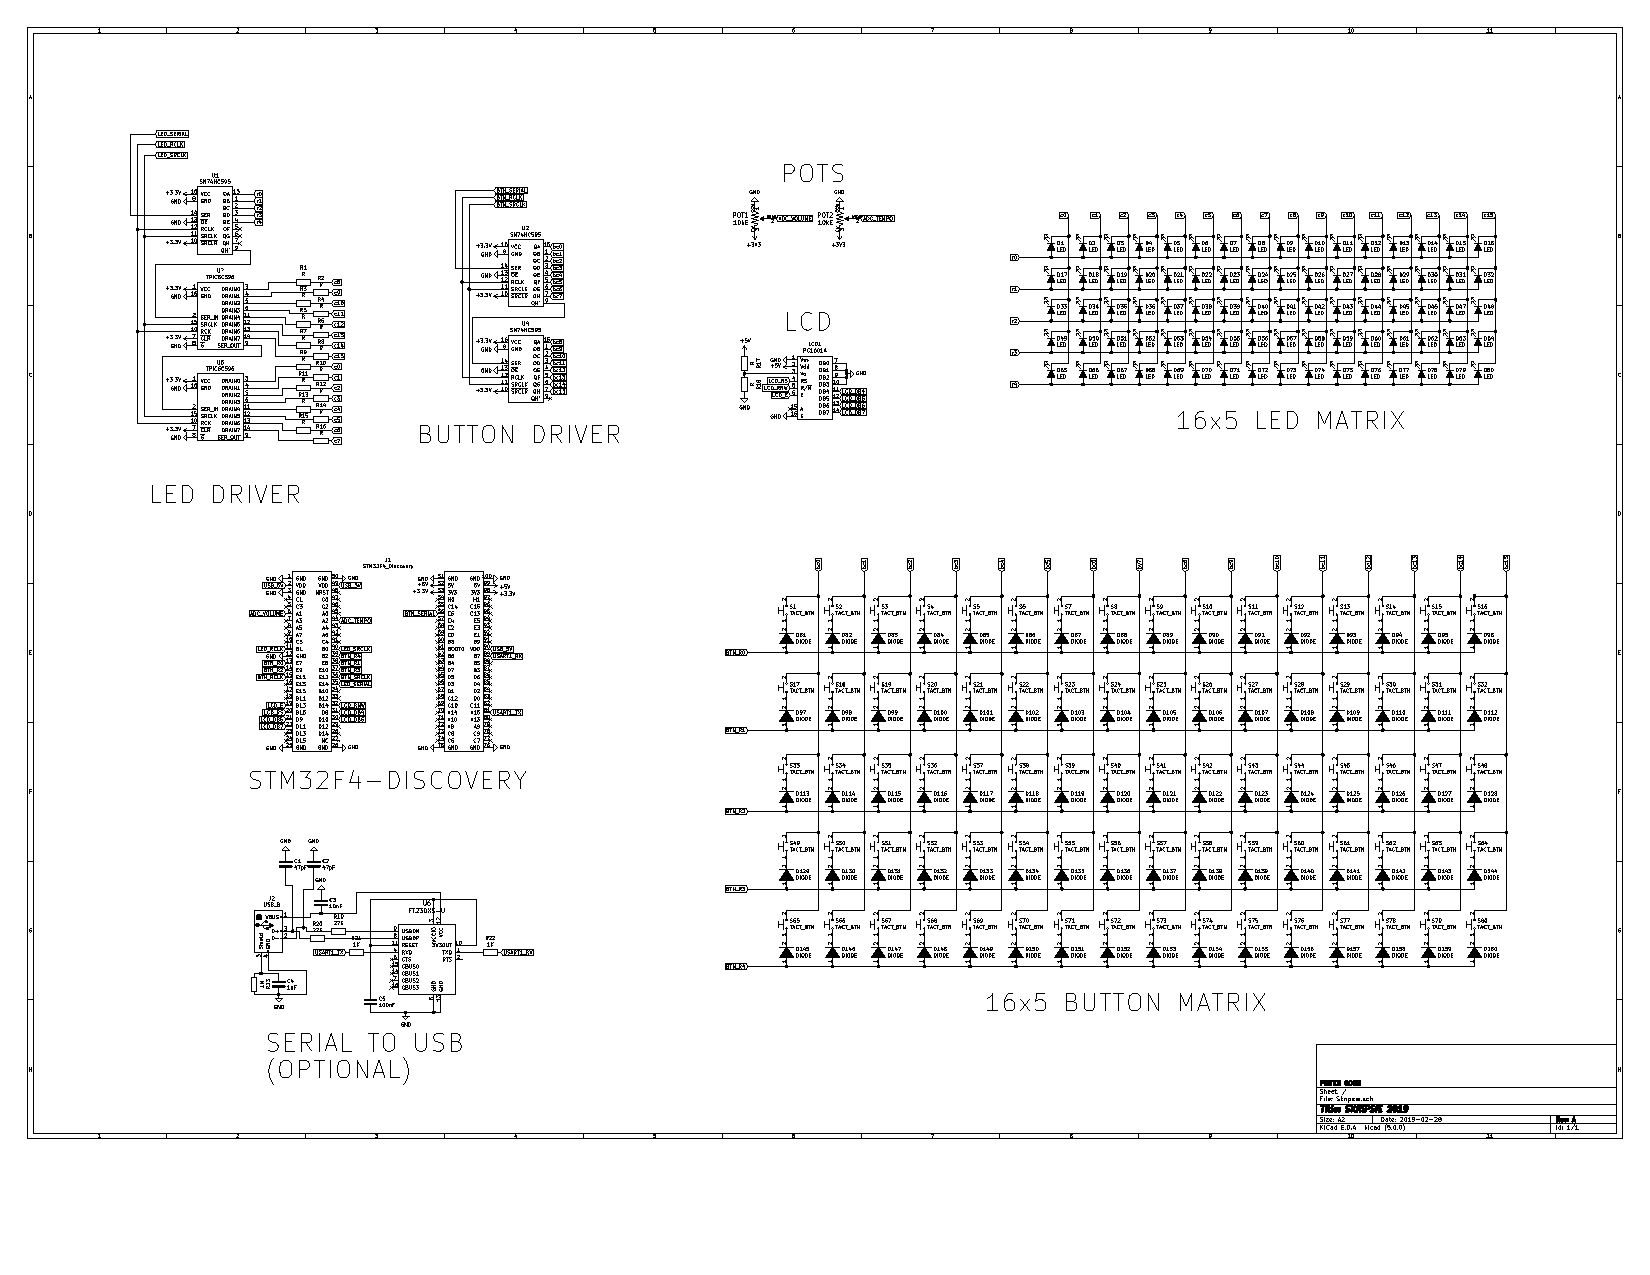
\includegraphics[width = \textwidth, angle=0, origin=c]{../Skripsie/Layout_28022019.pdf}
		\caption{Revision A of the Circuit Design}
	\end{center}
\end{figure}

\chapter{\ac{pcb} Design}
\begin{figure}[h!]
	\begin{center}
		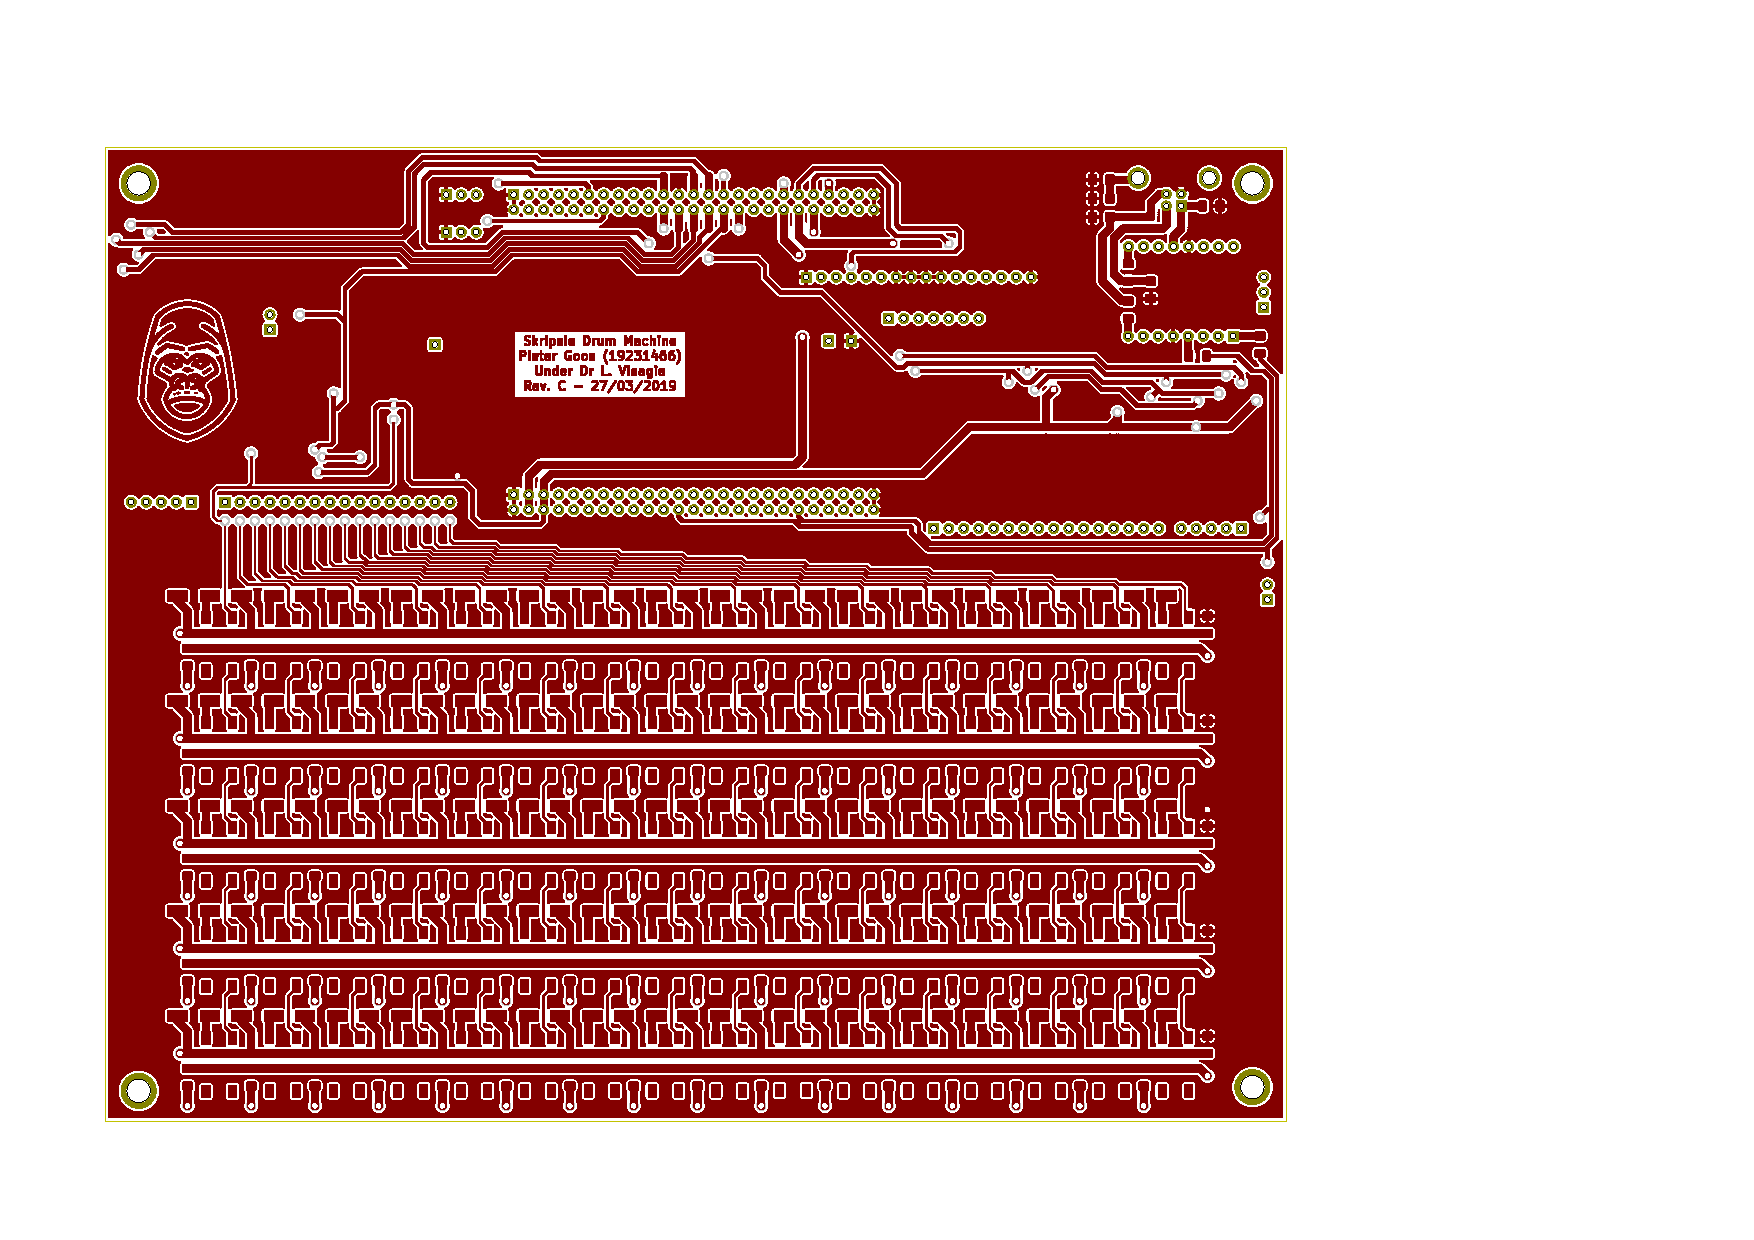
\includegraphics[width = \textwidth, trim={0.69in 0.78in 3.1in 0.95in}, clip]{../Skripsie/PCB_27032019.pdf}
		\caption{Front Copper Layer of Revision C of the \ac{pcb}}
		\label{fig:frontpcb}
	\end{center}
\end{figure}
\begin{figure}[h!]
	\begin{center}
		\includegraphics[page=2, width = \textwidth, trim={0.69in 0.78in 3.1in 0.95in}, clip]{../Skripsie/PCB_27032019.pdf}
		\caption{Back Copper Layer of Revision C of the \ac{pcb}}
		\label{fig:backpcb}
	\end{center}
\end{figure}

It is worth noting that this board (See Figures \ref{fig:frontpcb} and \ref{fig:backpcb}) shown is Revision C, however the board used to construct this project on is Revision B. The changes made between the two versions are simply forgotten traces, and mounting holes have been added.\\
When looking at the reverse of the board (As in Figure \ref{fig:backpcb}) it is worth noting that the shown diagram is not mirrored. This implies that the diagram shown's top left corner matches that of the front copper layer, thus one would have to mirror this from left to right to see what you would see in reality.

\newpage
\end{document}